\documentclass[xetex,dvipsnames,usenames]{beamer}

\frenchspacing

\usepackage[no-math]{fontspec}
\usepackage{xunicode}
\usepackage{xltxtra}


\setmainfont[Scale=MatchUppercase,Mapping=tex-text]{Fontin Sans}
\setsansfont[Scale=MatchLowercase,Mapping=tex-text, Numbers=OldStyle]{DaxCondensed}
\setmonofont[Scale=MatchLowercase]{Menlo}

\makeatletter

\setbeamercolor{block title}{use=structure,fg=structure.fg,bg=structure.fg!20!bg}
\setbeamercolor{block body}{parent=normal text,use=block title,bg=block title.bg!50!bg}
\AtBeginDocument{{\usebeamercolor{progressbar primary}}}

\defbeamertemplate*{footline}{}{
    \begin{beamercolorbox}[wd=\paperwidth,ht=0.8cm,dp=1ex]{progressbar inhead/foot}
        \hfill {\scriptsize \color{black!60} Xavier Olive -- ENSTA 2015 (IN104) {}}
    \end{beamercolorbox}}

\makeatother

\mode<presentation>
{
  \setbeamercovered{transparent}
  \setbeamertemplate{frametitle}{}
  \setbeamertemplate{blocks}[rounded][shadow=false]
  \setbeamertemplate{navigation symbols}{}
}

\graphicspath{{../../img/}}

\setbeamercolor{alerted text}{fg=BrickRed}

\begin{document}

\addtobeamertemplate{block begin}{\pgfsetfillopacity{0.7}}{\pgfsetfillopacity{1}}
\setbeamertemplate{background canvas}{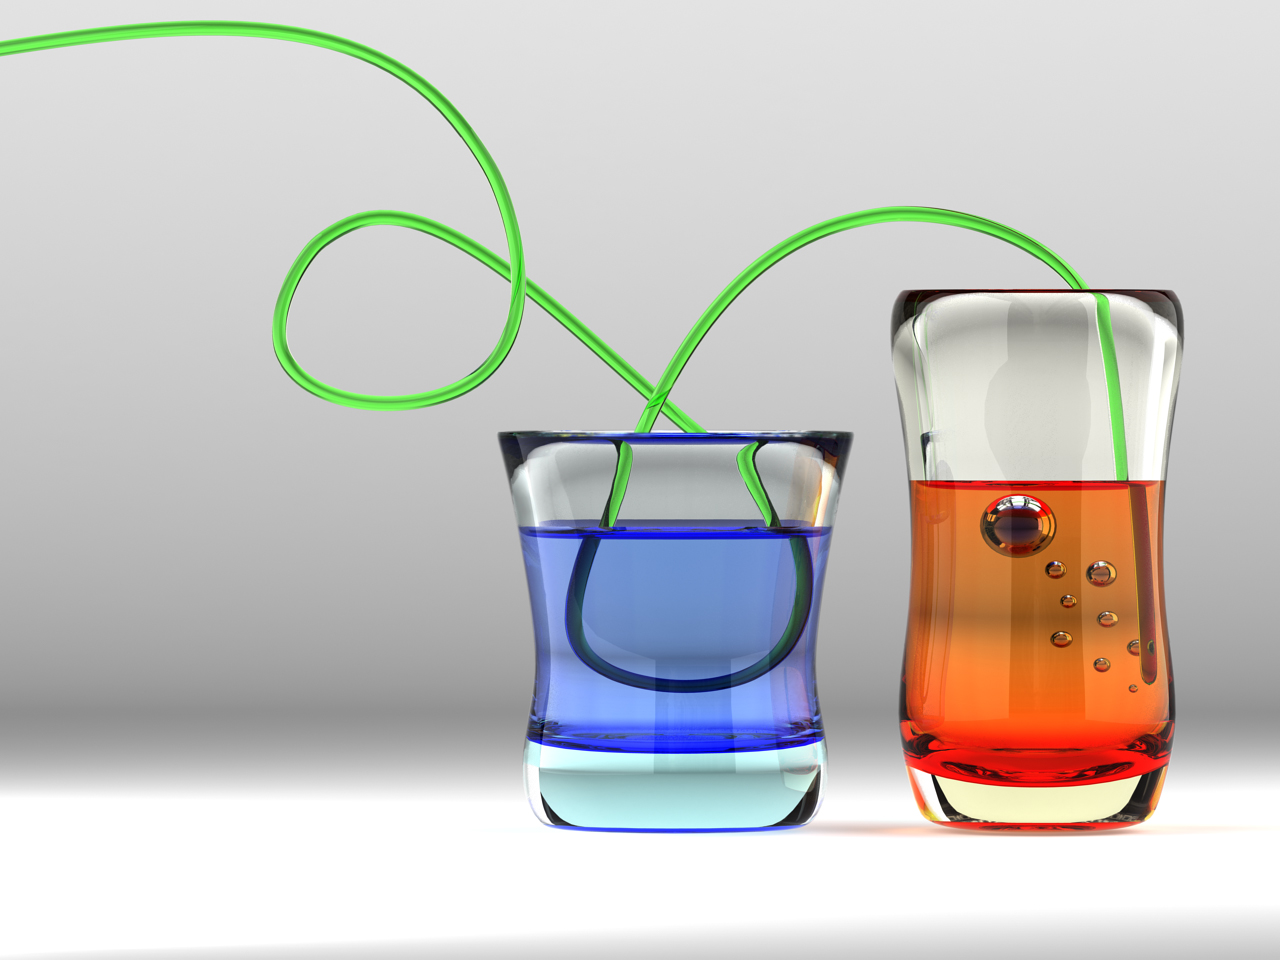
\includegraphics[width=\paperwidth]{glass_straw.png}}

\frame{
    \vspace{-2cm}
    \begin{block}{}
        \centerline{ \color{structure.fg}\Large Rendu d'images 3D par lancer de rayons}\vspace{5mm}
        Un \alert{algorithme performant} qui permet de rendre compte des caractéristiques
        géométriques de la lumière.
    \vspace{5mm}
    \end{block}
    \vfill
    \vspace{-3cm}
}

\setbeamertemplate{background canvas}{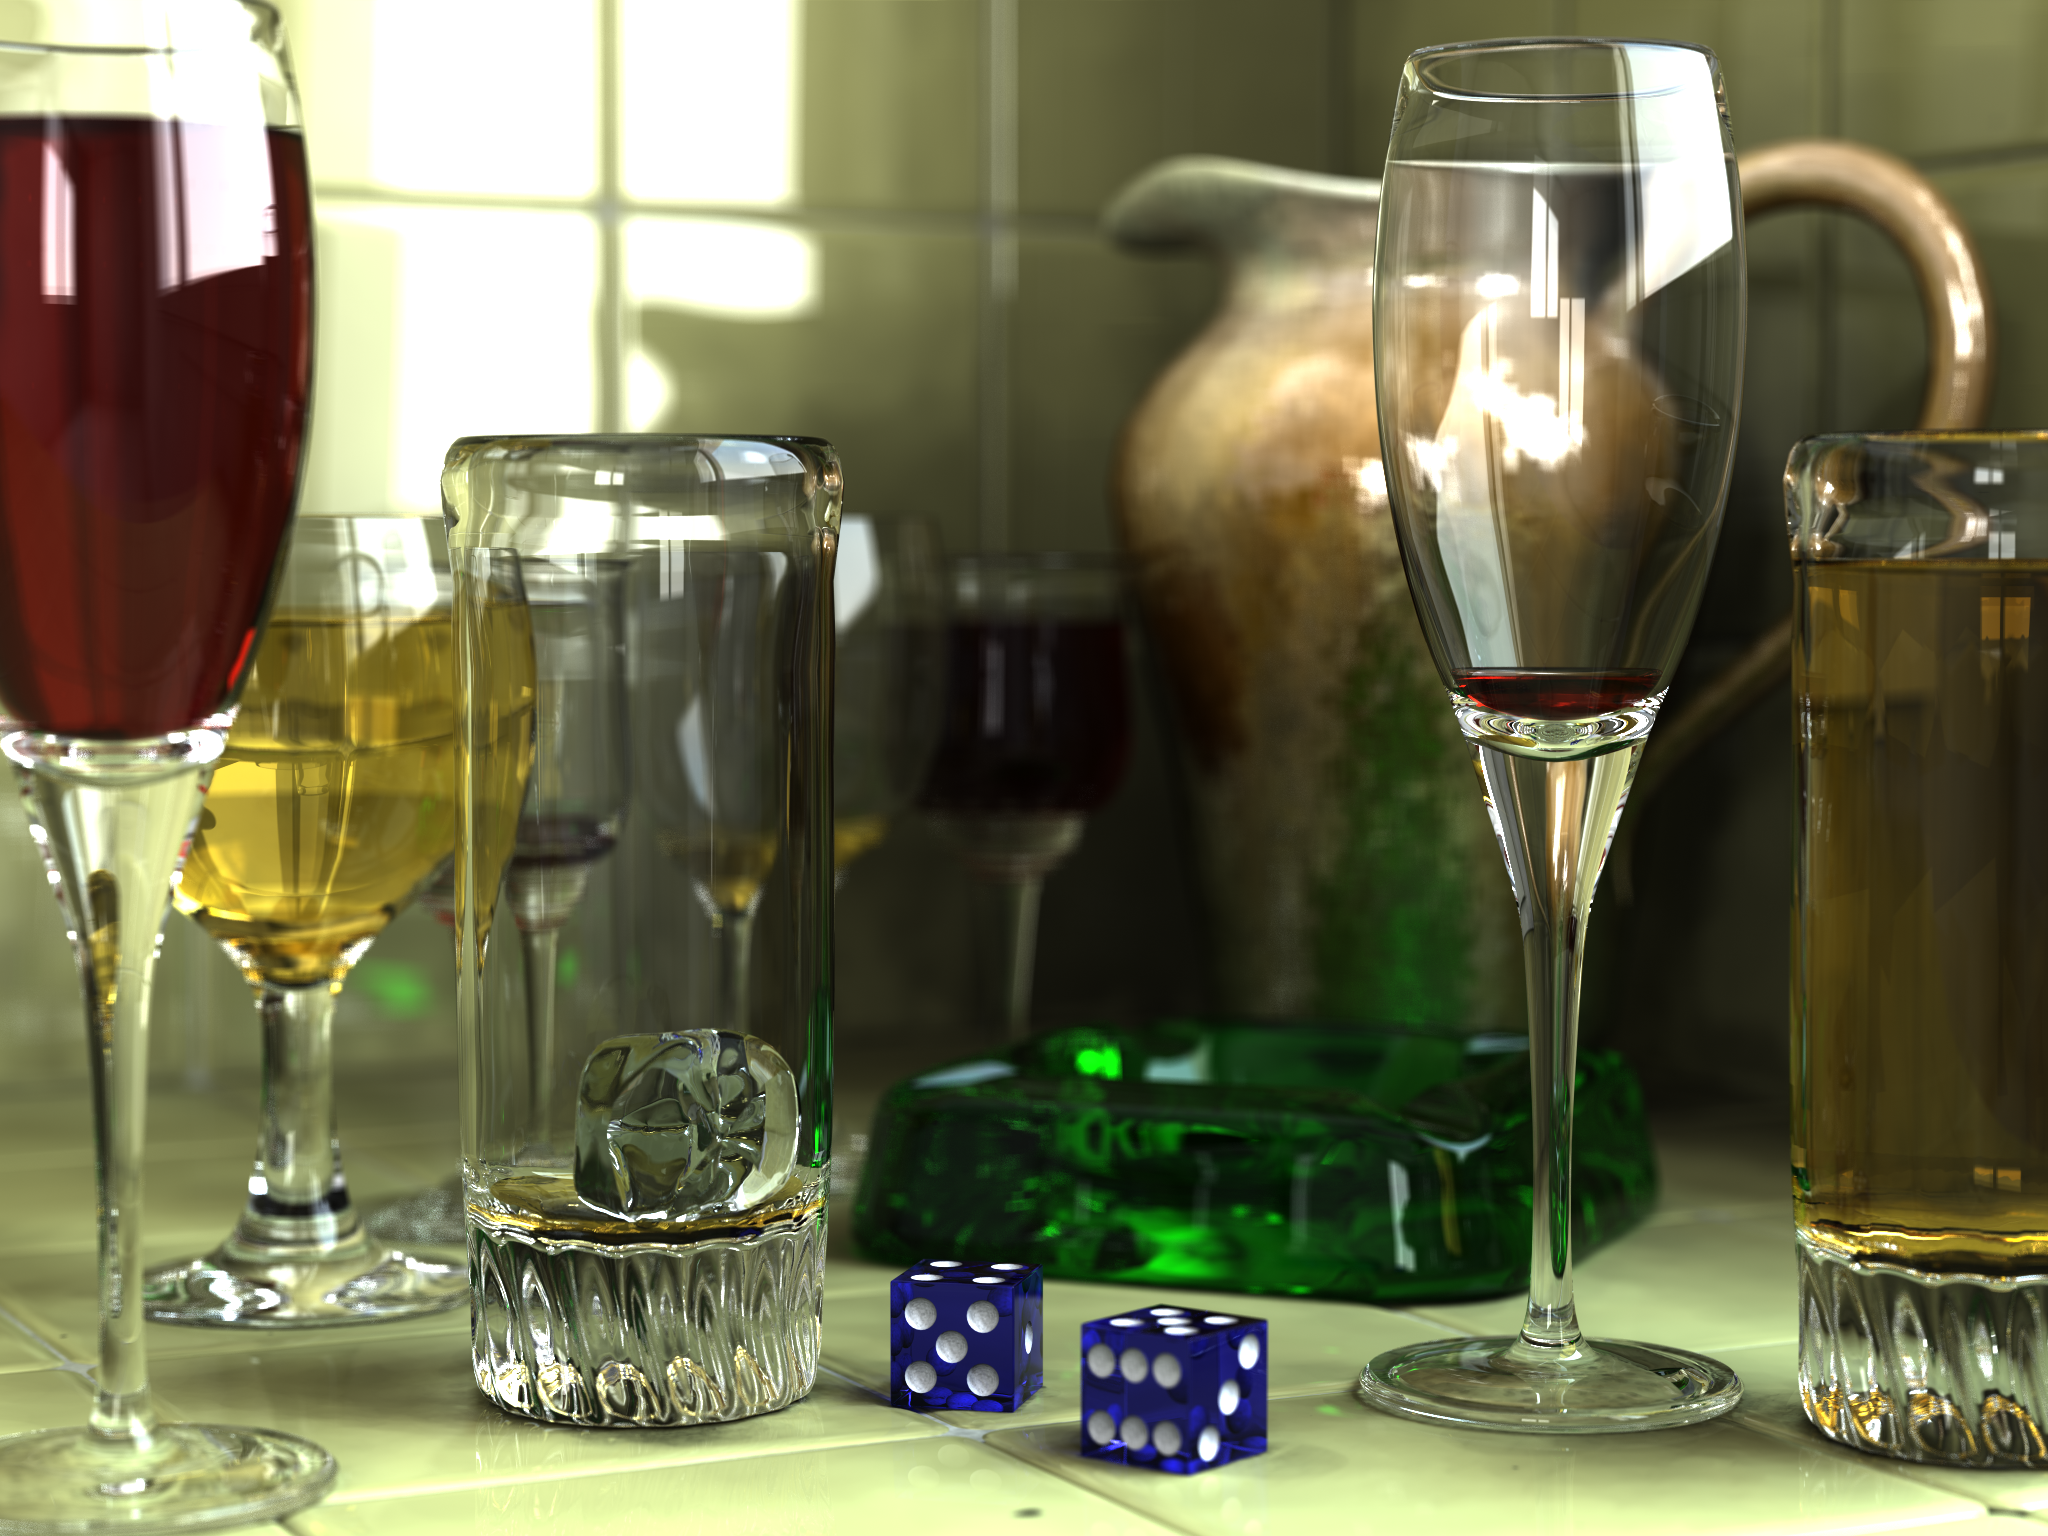
\includegraphics[width=\paperwidth]{glass_dice.png}}

\frame{
    \vfill
    \begin{block}
        {Principe}
    À partir d'une description d'un ensemble d'objets aux propriétés
    géométriques et visuelles différentes, on produit l'image que pourrait voir
    un observateur\\[2mm] en \alert{suivant le parcours inverse de la lumière}.
    \end{block}
    \vspace{-2cm}
}

\setbeamertemplate{background canvas}%
{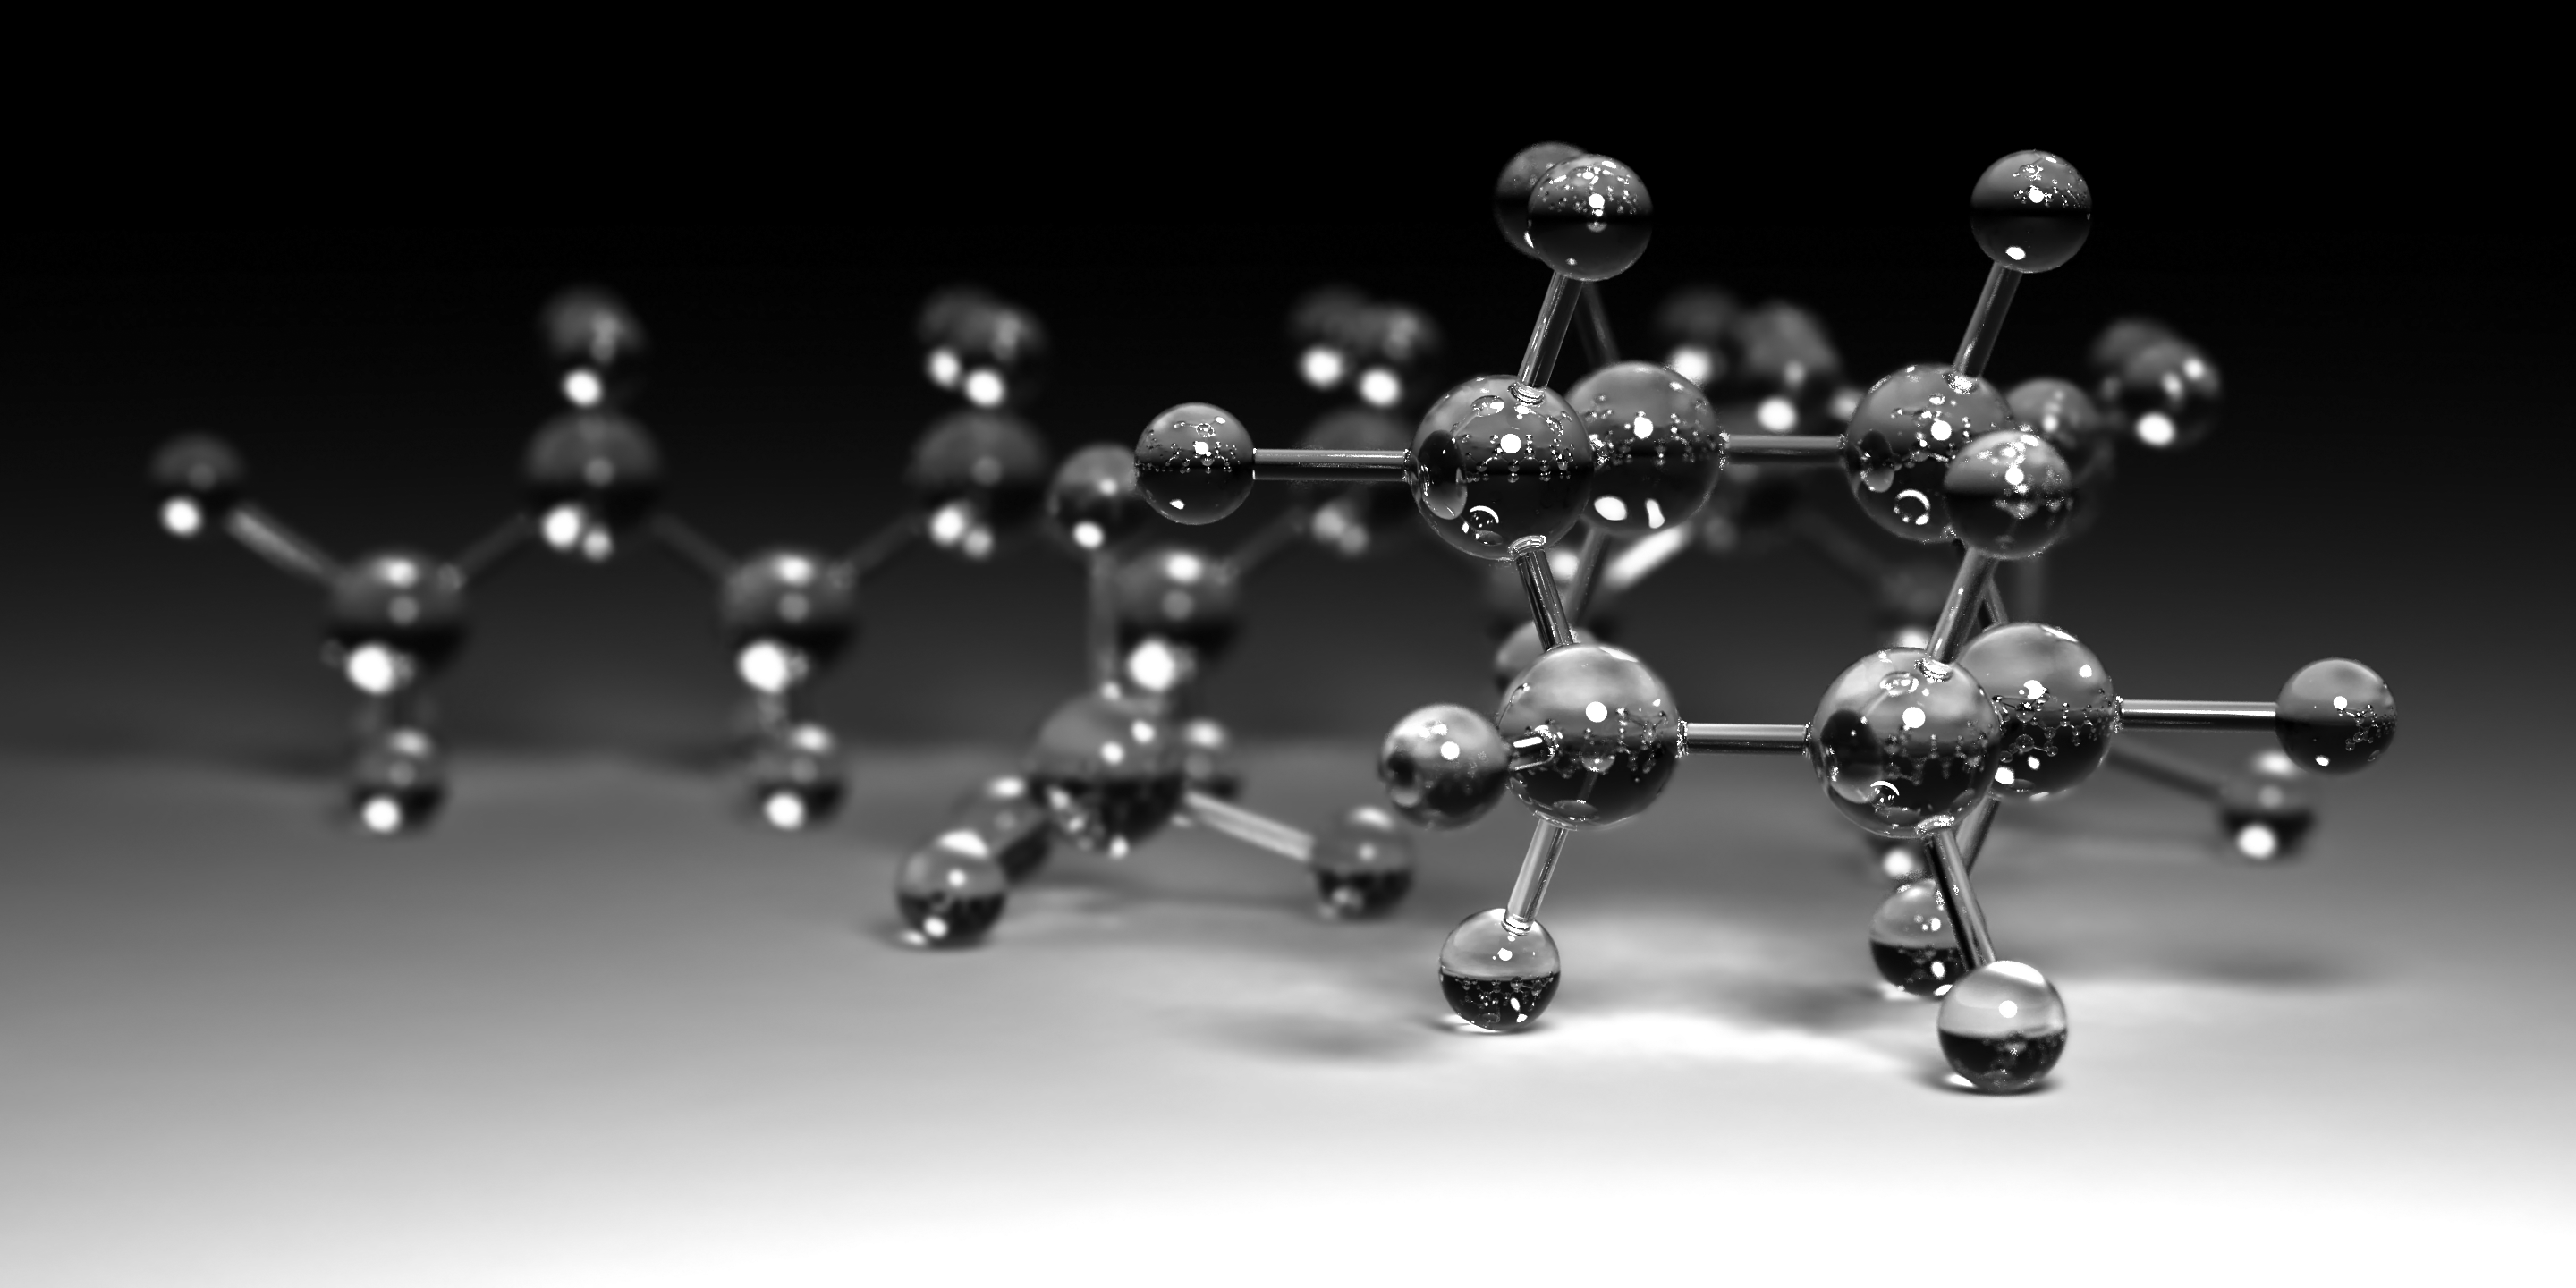
\includegraphics[width=\paperwidth]{molecules.png}}

\frame{
    \vfill
    \begin{block}
        {Objectifs}
        \begin{itemize}
            \item \alert{Concevoir, programmer et évaluer} un programme simple
                de rendu d'images 3D.
            \item Y \alert{prendre du plaisir}.
        \end{itemize}
    \end{block}
    \vspace{-3cm}
}

\setbeamertemplate{background canvas}%
{}

\frame{
    De la réfraction
    \vfill
    {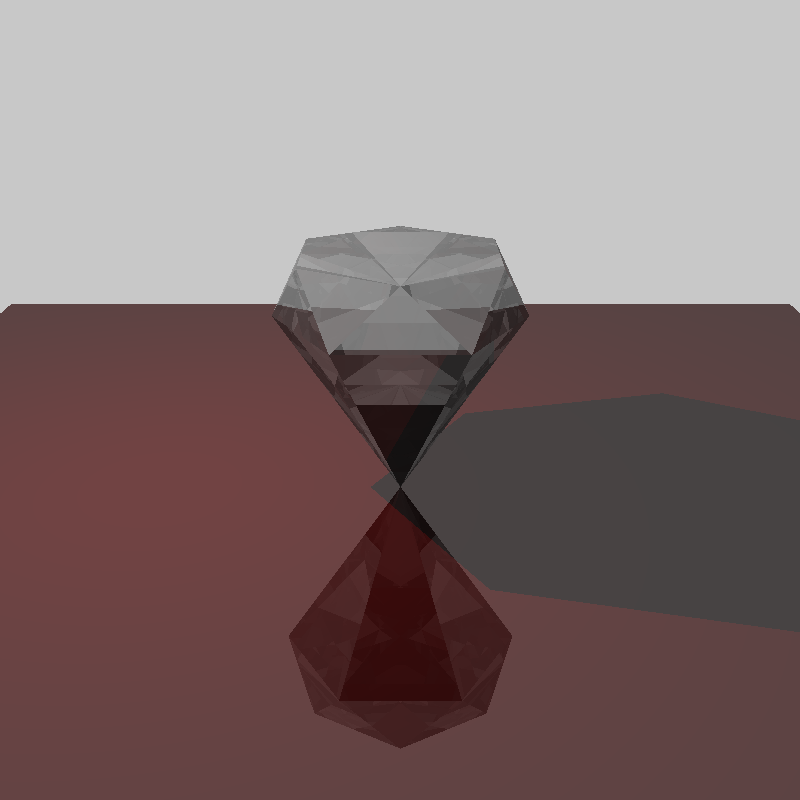
\includegraphics[width=.4\paperwidth]{bestof/diamant.png}}
    {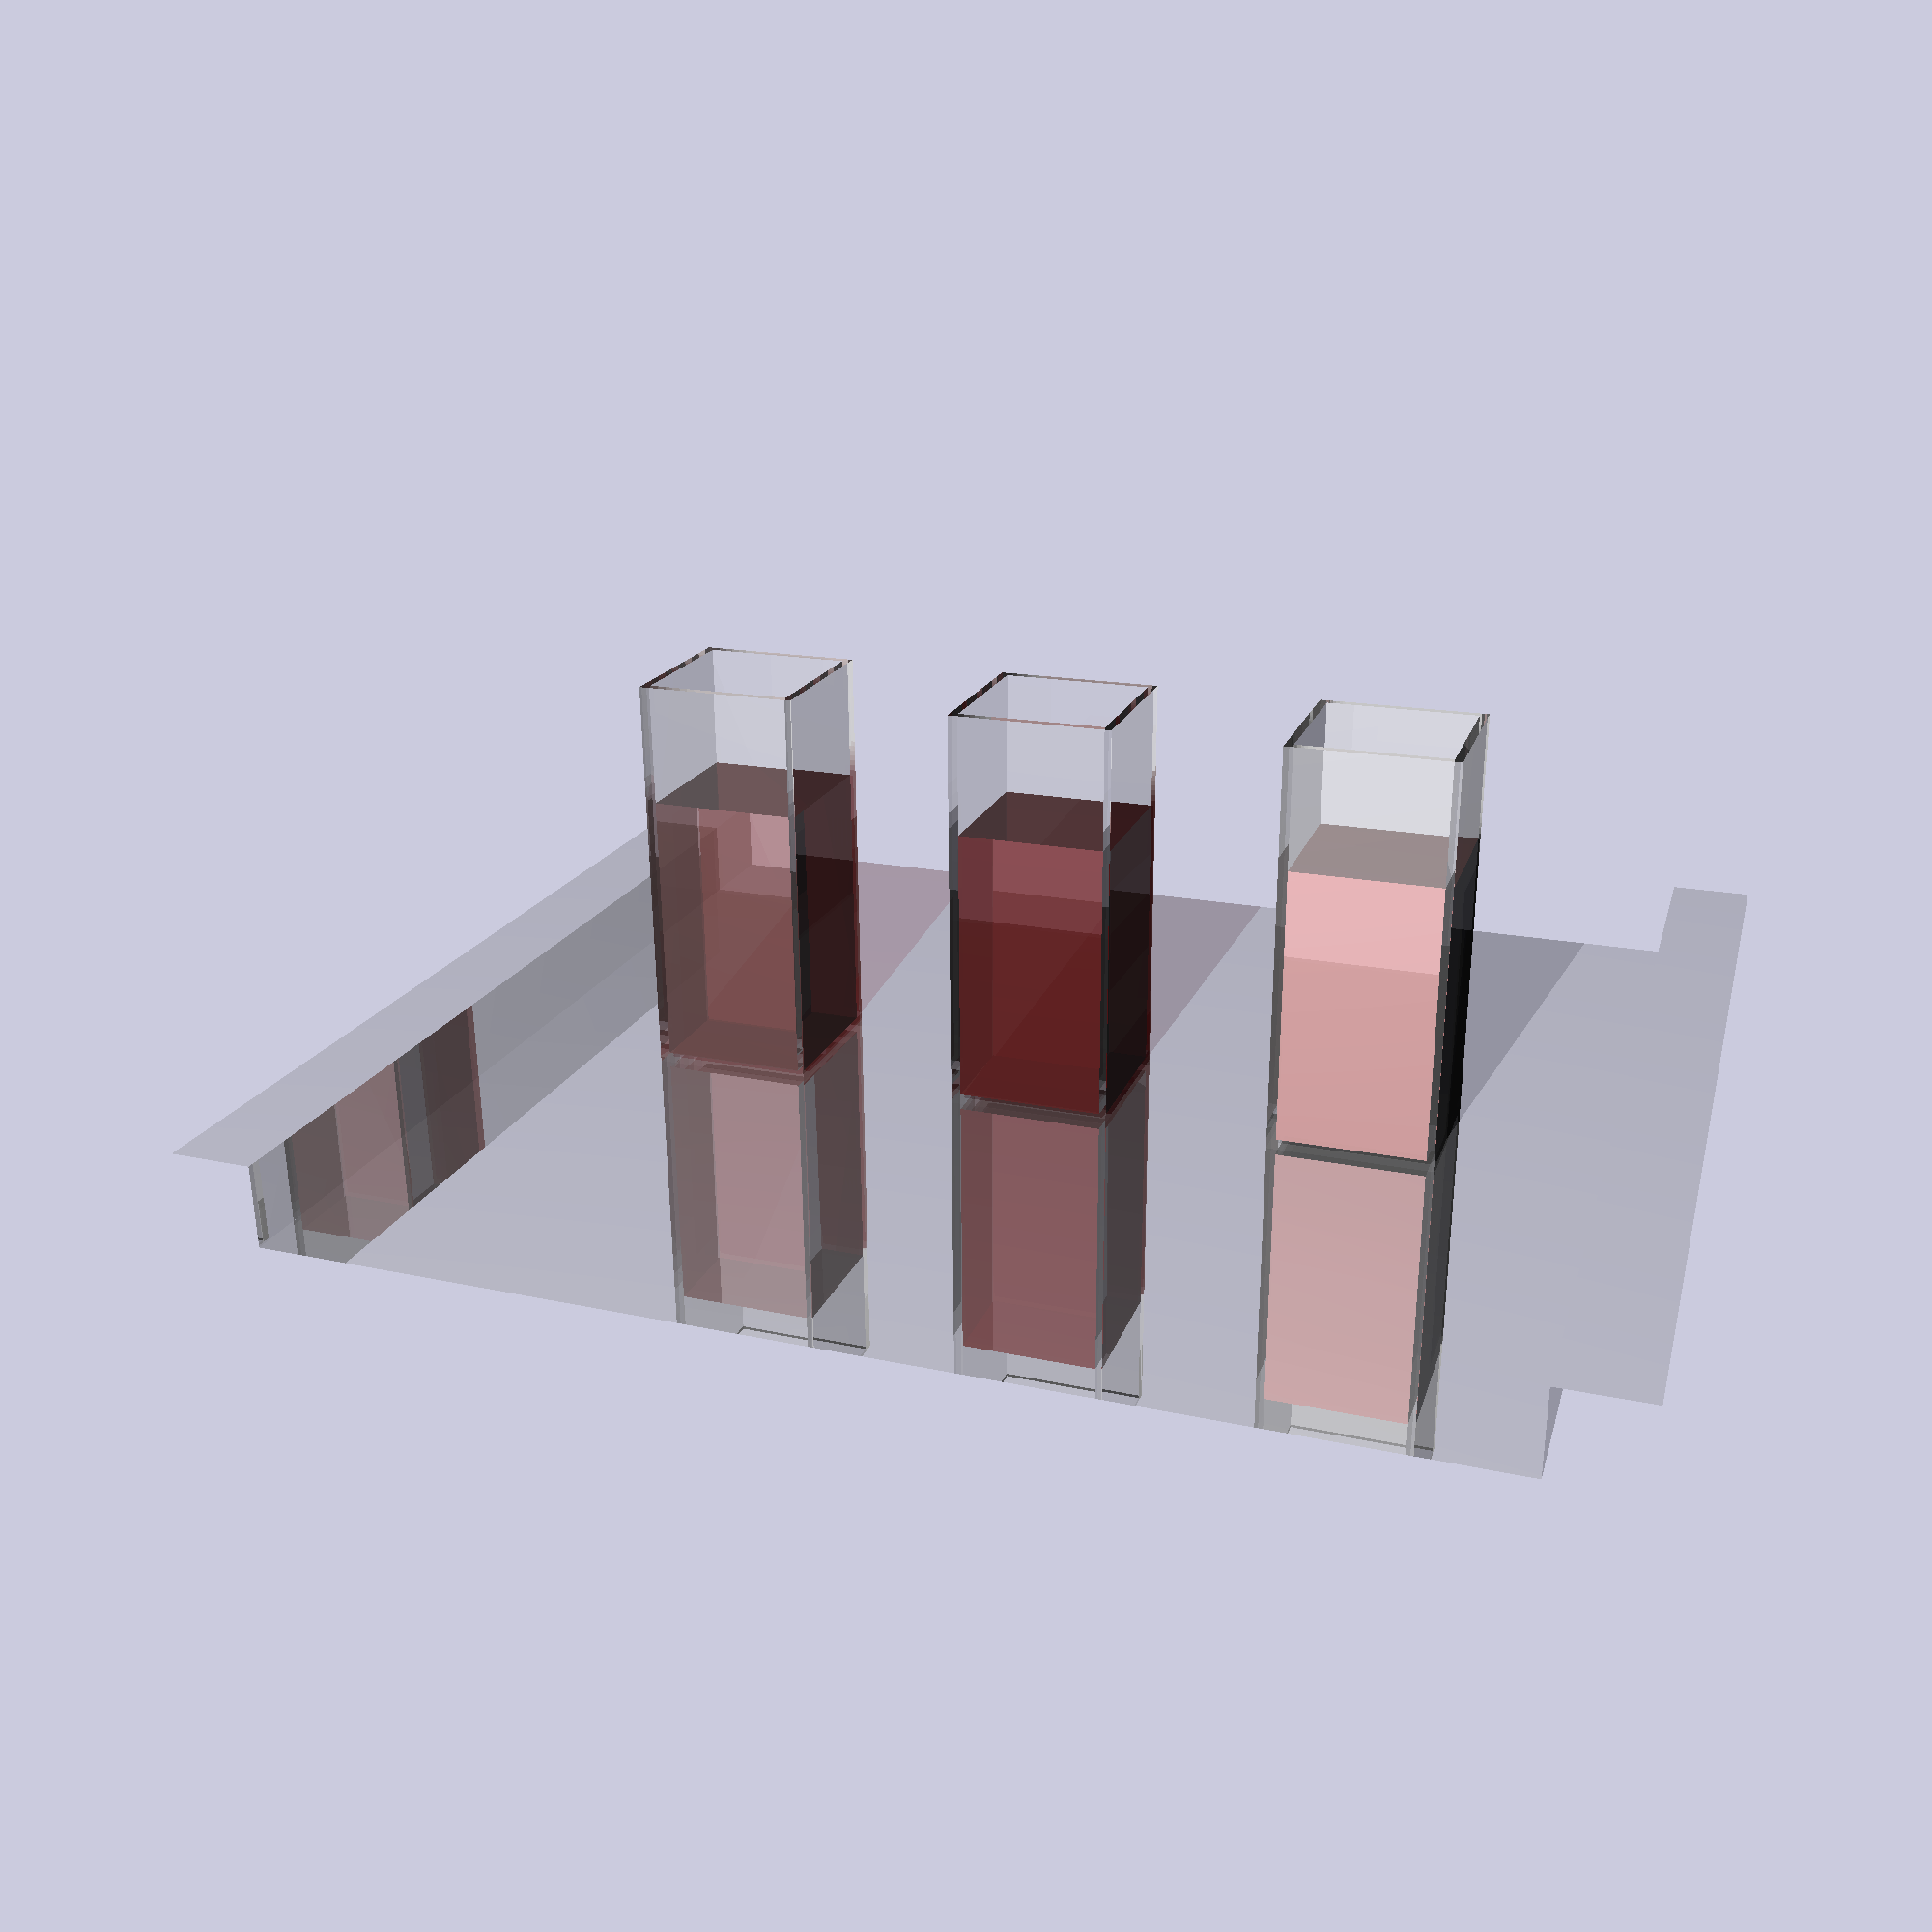
\includegraphics[width=.4\paperwidth]{bestof/verres.png}}
    \vfill
}

\frame{
    Des interférences
    \vfill
    {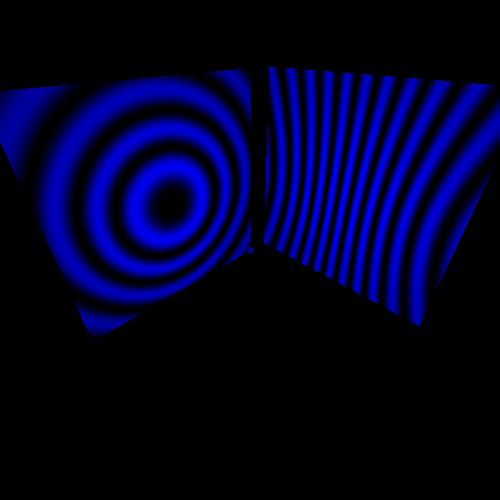
\includegraphics[width=.4\paperwidth]{bestof/michelson-bleu.png}}
    {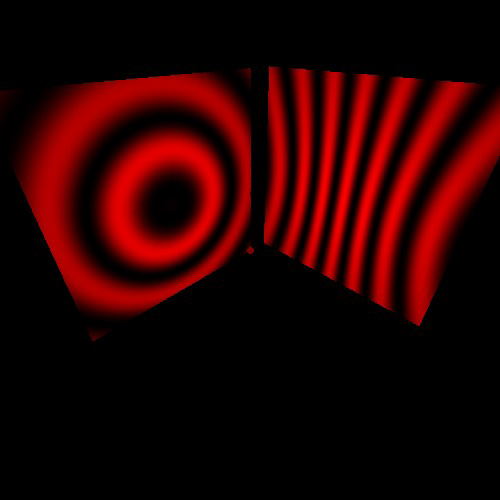
\includegraphics[width=.4\paperwidth]{bestof/michelson-rouge.png}}
    \vfill
}

\frame{
    Du flou de profondeur
    \vfill
    {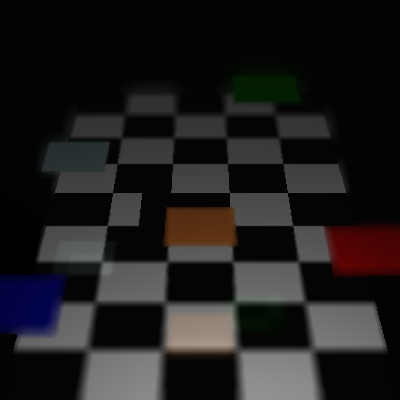
\includegraphics[width=.4\paperwidth]{bestof/focal-far.png}}
    {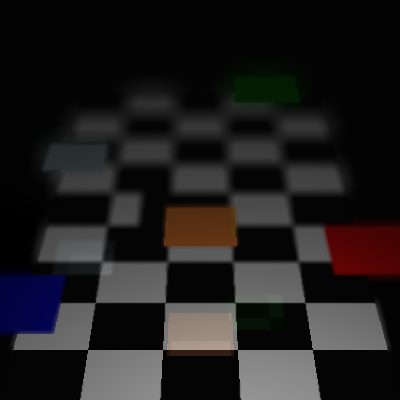
\includegraphics[width=.4\paperwidth]{bestof/focal-near.png}}
    \vfill
}

\frame{
    Et pour s'amuser avec des sphères\ldots
    \vfill
    {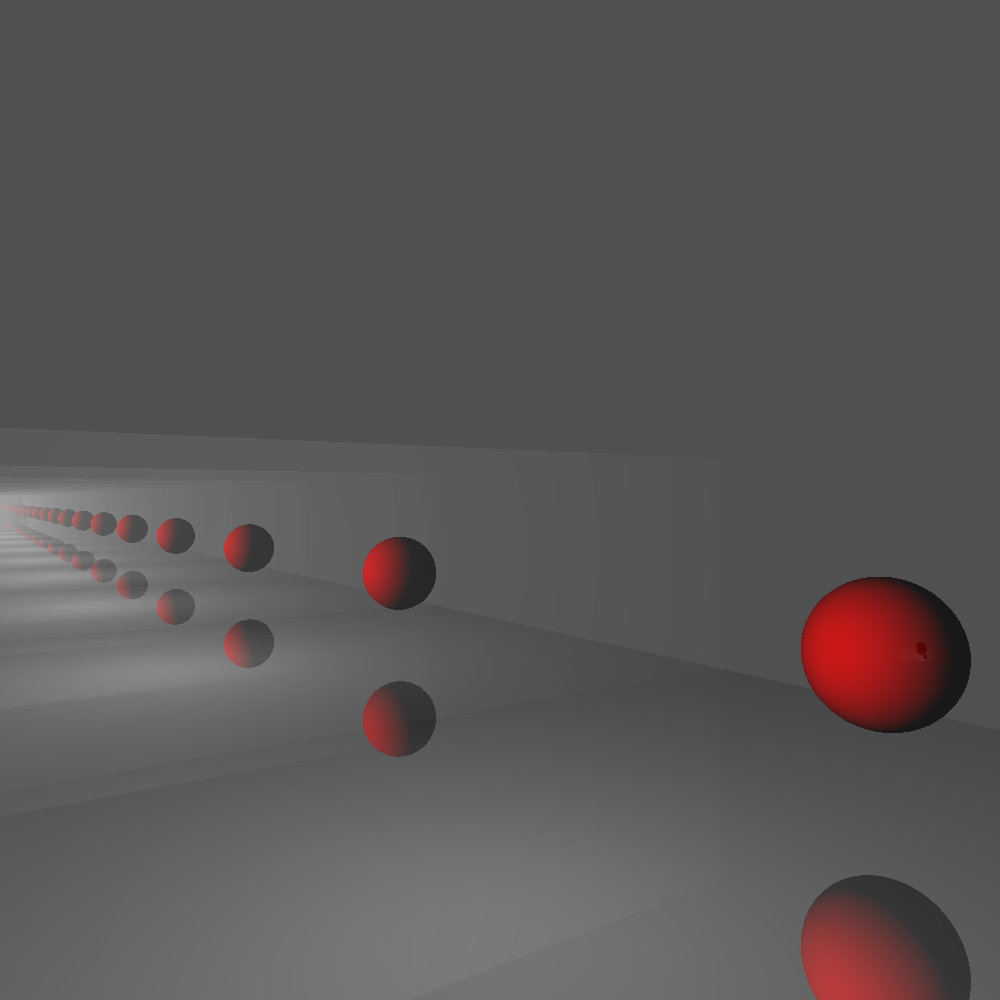
\includegraphics[width=.4\paperwidth]{bestof/sphere.png}}
    {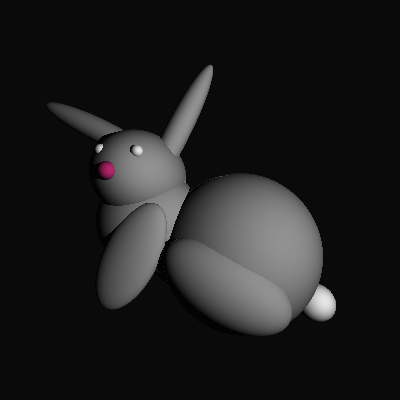
\includegraphics[width=.4\paperwidth]{bestof/lapin.png}}
    \vfill
}


\end{document}


